\begin{frame}[fragile]{Using UHD from C++ (1/5)}

\footnotesize

This section demonstrates how to develop and execute a C++ application using the
UHD C++ API to communicate with a USRP device.

\vspace{0.2cm}

\begin{itemize}
    \item \textbf{\textcolor{DarkBlue}{Step 1: Create a C++ Source File}}
\end{itemize}

\hspace{2.8em}
\parbox{0.88\linewidth}{
\footnotesize
Create a \texttt{.cpp} source file and write your UHD C++ application.
Typically, the application configures the USRP by setting and reading
parameters such as sampling rate, center frequency, gain, antenna,
clock source, etc.
}

\vspace{0.2cm}

\begin{itemize}
    \item \textbf{Code Explanation:}
\end{itemize}

\hspace{2.8em}
\scriptsize
\url{https://kb.ettus.com/Getting_Started_with_UHD_and_C%2B%2B}

%\vspace{0.3cm}

\begin{center}
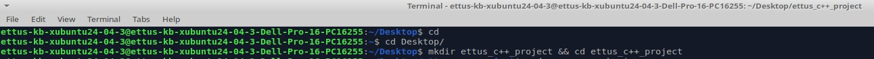
\includegraphics[height=0.08\textheight,keepaspectratio]
{latex/jpg_png/image_c++_1.png}

%\vspace{0.2cm}

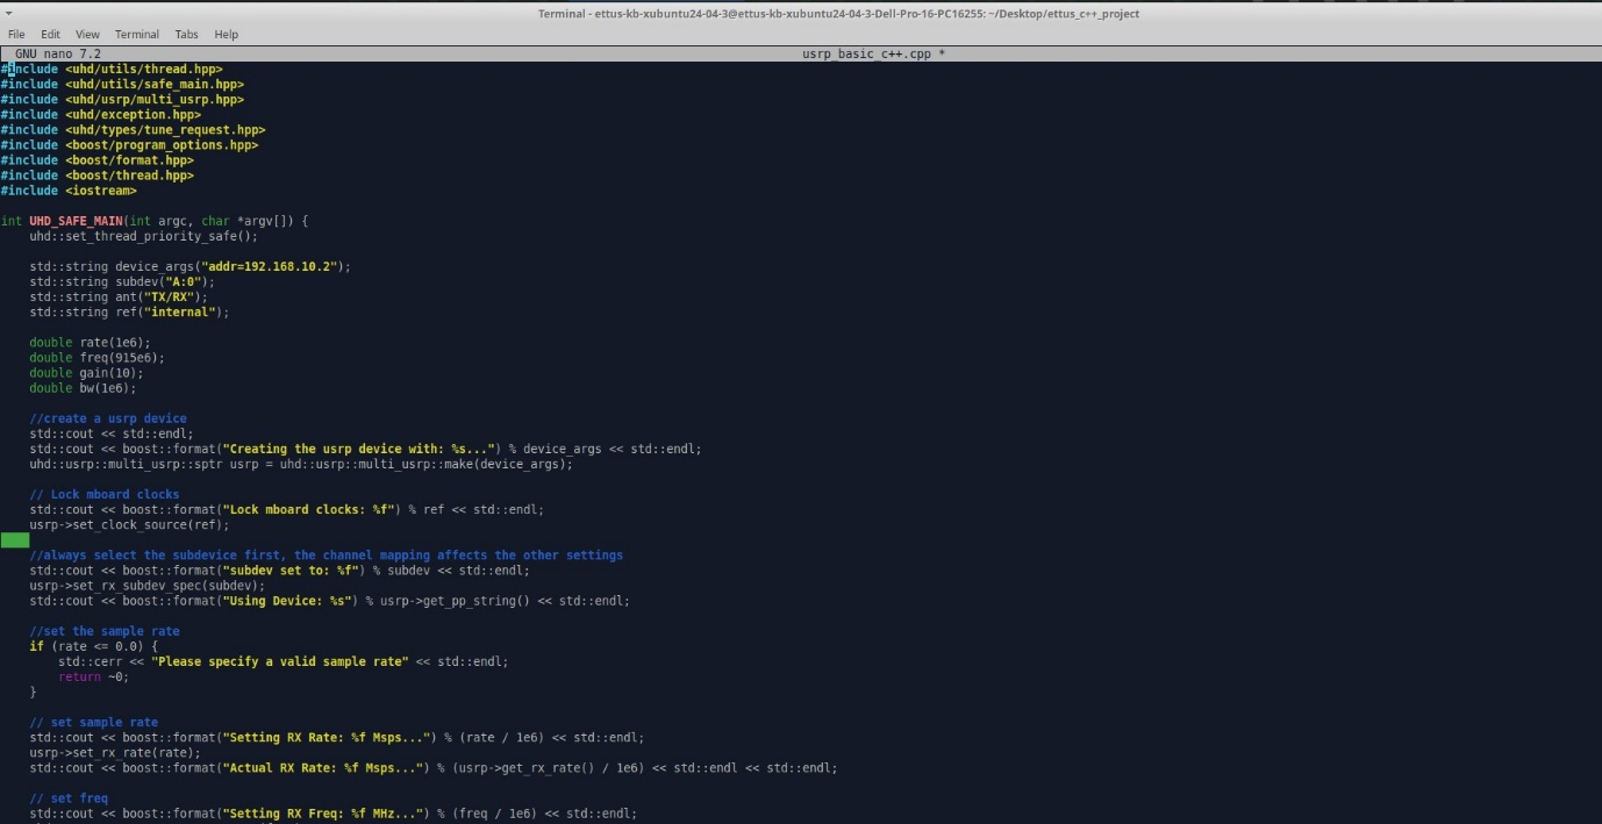
\includegraphics[height=0.42\textheight,keepaspectratio]
{latex/jpg_png/image_c++_2.png}
\end{center}

\end{frame}